% =====================================================================
%  Thesis C report -- Implementation chapter
%  Relative tracking of a car by a gimbal-camera quadcopter (DOPE + ArduPilot)
%
%  Compiles on its own (e.g. Overleaf, pdflatex). To use it inside your
%  thesis template, copy everything between "BEGIN CHAPTER" and
%  "END CHAPTER" into a chapter file and keep the \usepackage lines below
%  in your main preamble.
%
%  All numbers are measured values from the simulation logs
%  (logs/relative_pid_<timestamp>.csv, ArduPilot dataflash logs) and the
%  held-out DOPE test set; run identifiers are given where they are used.
% =====================================================================
\documentclass[11pt,a4paper]{report}
\usepackage[margin=25mm]{geometry}
\usepackage{amsmath,amssymb}
\usepackage{booktabs}
\usepackage{siunitx}
\usepackage{graphicx}
\usepackage{tikz}
\usetikzlibrary{arrows.meta,positioning,fit}
\usepackage{hyperref}
\sisetup{detect-all}

\begin{document}

% ------------------------------ BEGIN CHAPTER ------------------------------
\chapter{Implementation}
\label{ch:implementation}

This chapter describes the software and simulation system built to let a
quadcopter with a three-axis gimbal camera follow a moving car and hold a
cinematic shot position relative to it. The car is detected with a learned
6-DoF pose estimator (DOPE), its world-frame state is estimated from those
detections, and a relative-position controller sends velocity set-points to an
ArduPilot flight controller through MAVROS. Everything runs in a
software-in-the-loop (SITL) simulation in Gazebo, so the same ROS~2 nodes can
later run on a companion computer against real ArduPilot hardware.

\section{System overview}
\label{sec:overview}

Figure~\ref{fig:architecture} shows the processing chain. A gimbal camera image
is passed to the DOPE detector, which returns the car's pose in the camera
frame. The relative position controller transforms this pose into the world
frame, filters it into a car state estimate (position, velocity, heading and
yaw rate), computes the desired drone position from the active cinematic shot,
and outputs a velocity command. In parallel an image-space controller keeps the
car centred in the camera by commanding the gimbal. A flight sequencer handles
mode changes, arming, take-off and safety return-to-launch.

\begin{figure}[htbp]
  \centering
  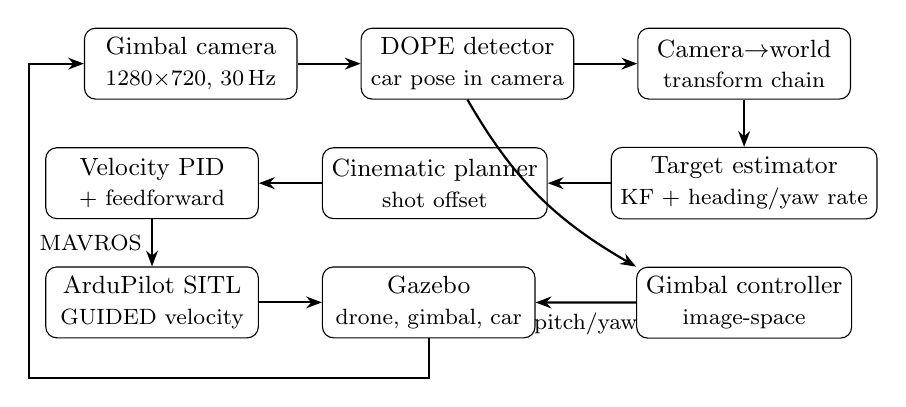
\begin{tikzpicture}[
      node distance=6mm and 8mm,
      blk/.style={draw, rounded corners, align=center, minimum height=9mm,
                  minimum width=27mm, font=\small},
      arr/.style={-{Stealth[length=2mm]}, thick}]
    \node[blk] (cam) {Gimbal camera\\\footnotesize 1280$\times$720, 30\,Hz};
    \node[blk, right=of cam] (dope) {DOPE detector\\\footnotesize car pose in camera};
    \node[blk, right=of dope] (frames) {Camera$\to$world\\\footnotesize transform chain};
    \node[blk, below=of frames] (est) {Target estimator\\\footnotesize KF + heading/yaw rate};
    \node[blk, left=of est] (plan) {Cinematic planner\\\footnotesize shot offset};
    \node[blk, left=of plan] (pid) {Velocity PID\\\footnotesize + feedforward};
    \node[blk, below=of pid] (ap) {ArduPilot SITL\\\footnotesize GUIDED velocity};
    \node[blk, right=of ap] (gz) {Gazebo\\\footnotesize drone, gimbal, car};
    \node[blk, below=of est] (gim) {Gimbal controller\\\footnotesize image-space};
    \draw[arr] (cam) -- (dope);
    \draw[arr] (dope) -- (frames);
    \draw[arr] (frames) -- (est);
    \draw[arr] (est) -- (plan);
    \draw[arr] (plan) -- (pid);
    \draw[arr] (pid) -- node[left, font=\footnotesize]{MAVROS} (ap);
    \draw[arr] (ap) -- (gz);
    \draw[arr] (dope.south) to[out=-60, in=150] (gim.north west);
    \draw[arr] (gim) -- node[below, font=\footnotesize]{pitch/yaw} (gz);
    \draw[arr] (gz.south) -- ++(0,-5mm) -| ([xshift=-7mm]cam.west) -- (cam.west);
  \end{tikzpicture}
  \caption{Processing chain of the tracking system.}
  \label{fig:architecture}
\end{figure}

\section{Simulation environment}
\label{sec:simulation}

\subsection{Software stack}
The simulation combines Gazebo Sim~10, ArduPilot SITL (ArduCopter) connected
through the \texttt{ardupilot\_gazebo} JSON plugin in lock-step mode, MAVROS as
the MAVLink bridge, and ROS~2. A single launch file starts all components in
separate terminals in a fixed order: Gazebo and the camera, clock and car
bridges at $t=0$, SITL after \SI{10}{s}, and MAVROS, the detector, the
controller and the operator GUI after \SI{40}{s}. The \SI{10}{s} delay was
introduced after a start-up deadlock was observed: when SITL connected before
Gazebo had initialised its renderer, the lock-step exchange stalled with SITL
re-sending the same servo frame (``No JSON sensor message received'') and the
plugin discarding it as a duplicate.

\subsection{Drone and gimbal model}
The drone is an Iris quadcopter with a three-axis gimbal (\texttt{gimbal\_small\_3d})
driven by ArduPilot's servo mount driver on servo channels 9--11. The camera on
the gimbal's pitch link was reconfigured to match the detector's camera model:
$1280\times720$ pixels, \SI{0.8}{rad} horizontal field of view and \SI{30}{Hz}.
The zoom plugin of the stock gimbal was removed so that the field of view
assumed by the detector cannot change.

An early version of the simulation loaded a model of the same name that had a
fixed, body-mounted camera and no gimbal joints, because Gazebo resolves
\texttt{model://} URIs in the world file's own directory first. ArduPilot's
servo mount has no angle feedback and reports the \emph{commanded} gimbal
attitude, so the controller believed the camera was moving when it was not.
This produced a car estimate \SI{17}{m} below the ground and, through the
velocity feedforward, a descent into the ground. The gimbal-equipped model
was therefore given a unique name (\texttt{iris\_with\_dope\_gimbal}).

Three ArduPilot parameter files are loaded on top of the defaults
(Table~\ref{tab:ardupilot-params}).

\begin{table}[htbp]
  \centering
  \caption{ArduPilot parameters changed from their defaults.}
  \label{tab:ardupilot-params}
  \begin{tabular}{@{}llp{75mm}@{}}
    \toprule
    Parameter & Value & Reason \\
    \midrule
    \texttt{MNT1\_DEFLT\_MODE} & 1 (Neutral) & default RC-targeting mode held the gimbal at \SI{-45}{\degree}, looking at the ground \\
    \texttt{MNT1\_NEUTRAL\_Y} & \SI{-5}{\degree} & camera sees a car \SI{20}{m} away both on the ground and after take-off \\
    \texttt{WP\_SPD} & \SI{15}{m/s} & guided-mode speed limit (default \SI{10}{m/s}) \\
    \texttt{WP\_ACC} & \SI{5}{m/s^2} & guided-mode acceleration limit (default \SI{2.5}{m/s^2}); needed to stay on the shot point in sharp turns \\
    Attitude tuning & softer rate loop & reduces camera vibration (\texttt{ATC\_RAT\_*}, \texttt{ATC\_INPUT\_TC}) \\
    \bottomrule
  \end{tabular}
\end{table}

MAVROS receives telemetry through MAVProxy, which re-requests all data streams
every \SI{15}{s} at its own rate (default \SI{4}{Hz}). At that rate the local
position arrived only every \SI{0.3}{s}; the stream rate was raised to
\SI{20}{Hz}.

\subsection{Target vehicle}
\label{sec:car-model}
The target is a model of an Audi R8 whose mesh is the same one used to render
the detector's training data. It was originally driven by a four-wheel
differential-drive plugin, which can turn on the spot and change speed
instantly. It was replaced by an Ackermann steering model with the real car's
dimensions (Table~\ref{tab:car}): rear-wheel drive, steered front wheels on
revolute knuckle joints, and a speed limiter so that the velocity is the
integral of a bounded, jerk-limited acceleration. A velocity command
$(v, \omega)$ is converted into a steering angle $\delta = \arctan(\omega L / v)$,
so the car only turns while it moves.

\begin{table}[htbp]
  \centering
  \caption{Target vehicle model (Ackermann steering).}
  \label{tab:car}
  \begin{tabular}{@{}lr@{}}
    \toprule
    Wheelbase $L$ & \SI{2.65}{m} \\
    Track / kingpin width & \SI{1.64}{m} / \SI{1.44}{m} \\
    Wheel radius & \SI{0.335}{m} \\
    Maximum wheel angle & \SI{0.5}{rad} (min.\ turning radius $\approx$ \SI{5.5}{m}) \\
    Maximum steering rate & \SI{1}{rad/s} \\
    Speed range & \SIrange{-8}{30}{m/s} \\
    Acceleration / braking / jerk limit & \SI{3}{m/s^2} / \SI{6}{m/s^2} / \SI{15}{m/s^3} \\
    \midrule
    \multicolumn{2}{@{}l}{\emph{Measured in Gazebo}} \\
    Turn command at standstill & no motion \\
    \SIrange{0}{8}{m/s} & $\approx$ \SI{2.7}{s} (peak \SI{3.3}{m/s^2}) \\
    \SI{8}{m/s} with \SI{0.4}{rad/s} commanded & \SIrange{21}{22}{\degree\per\second} achieved \\
    Stop from \SI{8}{m/s} & $\approx$ \SI{2}{s} (peak \SI{4.9}{m/s^2}) \\
    \bottomrule
  \end{tabular}
\end{table}

\section{Perception: DOPE pose estimation}
\label{sec:perception}

\subsection{Detector}
DOPE (Deep Object Pose Estimation) predicts belief maps for the eight corners
and the centroid of the object's 3-D bounding cuboid; the pose is then recovered
with a PnP solver using the known cuboid dimensions
($203.8\times124.0\times441.5$\,cm). The detector node runs the network on the
latest camera frame only (no backlog), at up to \SI{20}{Hz}, and publishes the
car pose in the OpenCV camera frame together with the image capture time stamp.

\subsection{Training data}
Training images were rendered with BlenderProc using the same car mesh, random
distractor objects and HDRI backgrounds. The data generator was modified to
place the car at a true camera-to-object distance sampled log-uniformly between
a near and far limit, and to orient it so that the camera looks down on it from
a drone-like elevation with a level horizon (Table~\ref{tab:datasets}).

Detection losses in flight were analysed by projecting the true car cuboid into
the camera image: in two runs every lost frame had part of the car outside the
image, at \SIrange{4}{9}{m} range or \SIrange{59}{89}{\degree} look-down,
whereas no frame with the whole car in view was lost. The earlier training
sets only contained views between \SIrange{3}{75}{\degree} elevation and
\SIrange{7}{45}{m}, always with the whole car in frame, so two further sets
targeting these cases were generated.

\begin{table}[htbp]
  \centering
  \caption{Rendered training and test data (Audi R8).}
  \label{tab:datasets}
  \begin{tabular}{@{}lrlll@{}}
    \toprule
    Set & Frames & Look-down & Distance & Purpose \\
    \midrule
    v1 & 300 & \SIrange{5}{75}{\degree} & \SIrange{7}{45}{m} & first drone-view set \\
    v2 & 3000 & \SIrange{3}{75}{\degree} & \SIrange{7}{45}{m} & main set \\
    v3 overhead & 1200 & \SIrange{55}{89}{\degree} & \SIrange{6}{20}{m} & nearly overhead views \\
    v3 close & 1200 & \SIrange{20}{89}{\degree} & \SIrange{4}{10}{m} & car partly out of frame \\
    Test (held out) & $3\times150$ & overhead / close / standard & & evaluation only \\
    \bottomrule
  \end{tabular}
\end{table}

The v3 model was fine-tuned from the v2 weights for 100 epochs on all four
training sets (5700 frames, batch size 32, image size 448, learning rate
$10^{-4}$), taking about \SI{60}{s} per epoch on one GPU.

\subsection{Evaluation}
Each model was evaluated on the held-out test set (Table~\ref{tab:dope-eval}). The pose is compared with
the ground truth after converting the renderer's camera frame (x right, y up,
z backwards) into the OpenCV frame; the keypoint error is the mean pixel
distance between the nine reprojected cuboid points and the ground-truth
projections, and a keypoint error above \SI{25}{px} is counted as an
orientation flip (e.g.\ front and back confused).

\begin{table}[htbp]
  \centering
  \caption{DOPE models on the held-out test set (150 frames per view type).}
  \label{tab:dope-eval}
  \begin{tabular}{@{}lcccc@{}}
    \toprule
     & \multicolumn{2}{c}{v2 (epoch 725)} & \multicolumn{2}{c}{v3 (epoch 850)} \\
    \cmidrule(lr){2-3}\cmidrule(l){4-5}
    Test set & detected & flips & detected & flips \\
    \midrule
    Overhead (\SIrange{55}{89}{\degree}, \SIrange{6}{20}{m}) & 93\,\% & 1\,\% & 98\,\% & 0\,\% \\
    Close (\SIrange{20}{89}{\degree}, \SIrange{4}{10}{m}) & 56\,\% & 6\,\% & 65\,\% & 0\,\% \\
    Standard (\SIrange{3}{75}{\degree}, \SIrange{7}{45}{m}) & 99\,\% & 1\,\% & 99\,\% & 0\,\% \\
    \bottomrule
  \end{tabular}
\end{table}

The median position error was about \SI{0.6}{m} and the keypoint error about
\SI{5}{px} for both models. On the close-range set the remaining misses are
explained by visibility: with all eight corners in the image both models detect
the car in every frame, with 4--5 corners visible v3 detects 75\,\% (v2 54\,\%),
and with three or fewer corners neither model detects it. Since a
cuboid-keypoint method needs enough visible corners, this limit is addressed by
keeping the drone at least \SI{10}{m} from the car
(Section~\ref{sec:planner}) rather than by more training.

\section{Camera-to-world transformation}
\label{sec:frames}

A detection gives the car pose $\mathbf{T}_{C}^{\,car}$ in the camera optical
frame $C$ (x right, y down, z forward). Its world pose is obtained through the
chain
\begin{equation}
  \mathbf{T}_{W}^{\,car} =
  \mathbf{T}_{W}^{\,B}\,\mathbf{R}_{FLU}^{\,FRD}\,
  \mathbf{T}_{FRD}^{\,G}\,\mathbf{T}_{G}^{\,C}\,\mathbf{T}_{C}^{\,car},
  \label{eq:chain}
\end{equation}
where $\mathbf{T}_{W}^{\,B}$ is the drone pose from MAVROS (ENU world, FLU body),
$\mathbf{R}_{FLU}^{\,FRD}=\operatorname{diag}(1,-1,-1)$,
$\mathbf{T}_{FRD}^{\,G}$ is the gimbal attitude reported by ArduPilot, and
$\mathbf{T}_{G}^{\,C}$ maps the gimbal's forward-right-down axes onto the
optical axes. The drone pose and gimbal attitude are kept in short histories so
that the values at the image capture time can be used.

The frame in which the gimbal attitude is expressed was determined
experimentally. The MAVLink status flags of ArduPilot's servo mount suggest a
horizon-referenced roll and pitch, but over 111 logged detections the reported
gimbal pitch equalled the commanded pitch plus the drone's pitch (correlation
0.94), i.e.\ it is body-referenced. Treating it as horizon-referenced applied the
drone's tilt twice: the vertical error of the car's image position followed the
drone pitch with a slope of $-0.97$ (correlation 0.95), with a mean error of
\SI{14}{\degree} and a maximum of \SI{31}{\degree}. With the body-frame
interpretation of Equation~\eqref{eq:chain} the estimate of a parked car stabilised
(Table~\ref{tab:gimbal-frame}).

\begin{table}[htbp]
  \centering
  \caption{Parked-car estimate before and after correcting the gimbal attitude frame.}
  \label{tab:gimbal-frame}
  \begin{tabular}{@{}lcc@{}}
    \toprule
     & horizon frame & body frame \\
    \midrule
    Estimated car height & \SIrange{-7}{14}{m} & $0.71\pm0.22$\,m \\
    Position error (along line of sight) & up to \SI{8}{m} & $-0.20\pm0.24$\,m \\
    Heading error & -- & $-0.3\pm3.7$\,\si{\degree} \\
    Vertical command at its $\pm$\SI{3}{m/s} limit & almost every cycle & never \\
    \bottomrule
  \end{tabular}
\end{table}

\section{Target state estimation}
\label{sec:estimation}

\paragraph{Gating.}
A detection is rejected if its range lies outside \SIrange{0.2}{80}{m} or if its
world position is further than $3 + 0.1\,r$\,m ($r$ the range) from the Kalman
filter prediction. After five consecutive rejections the next detection is
accepted and the filters are re-initialised, so a filter that locked onto a
wrong value cannot exclude the target permanently.

\paragraph{Position and velocity.}
A linear constant-velocity Kalman filter with state
$\mathbf{x}=[p_x,p_y,p_z,v_x,v_y,v_z]^\top$ and white-noise acceleration
($\sigma_a=\SI{1.5}{m/s^2}$) filters the world positions. The measurement
noise grows with range, $\sigma_r = 0.15 + 0.02\,r$\,m, and the process noise is
adapted to the normalised innovation. The time step is taken from the image
capture stamps so that detection latency jitter does not appear as acceleration.

\paragraph{Heading and yaw rate.}
The heading $\psi$ is the world yaw of the car's forward axis in the detected pose.
It is filtered with a jump-gated circular exponential moving average
($\alpha=0.25$; jumps above \SI{60}{\degree} are rejected unless they persist).
The yaw rate is the low-pass filtered derivative of the filtered heading,
\begin{equation}
  \hat\omega_k = \hat\omega_{k-1} + \frac{\Delta t}{\tau+\Delta t}
  \left(\frac{\operatorname{wrap}(\hat\psi_k-\hat\psi_{k-1})}{\Delta t}-\hat\omega_{k-1}\right),
  \qquad \tau = \SI{1}{s},
\end{equation}
and is faded to zero below a speed of \SI{1}{m/s} (full above \SI{2}{m/s}),
because a car cannot turn in place and heading noise on a parked car would
otherwise appear as a turn rate. A constant-turn-rate-and-velocity UKF was also
implemented; it was made numerically robust (all sigma-point weights positive,
symmetrised covariance) but with detector-level noise it flipped its heading by
\SI{180}{\degree} in turns and is disabled.

\section{Drone control}
\label{sec:control}

\subsection{Shot point and feedforward}
The cinematic planner provides a shot offset $\mathbf{o}=(o_x,o_y,o_z)$ in the car
frame (x forward, y left). The desired drone position is
\begin{equation}
  \mathbf{p}_d = \hat{\mathbf{p}}_{car} + \mathbf{R}(\hat\psi + \hat\omega\,t_p)\,
  \begin{bmatrix}o_x\\ o_y\end{bmatrix},\qquad
  z_d = z_{ground} + o_z ,
\end{equation}
where the heading is predicted $t_p=\SI{0.35}{s}$ ahead to compensate the heading
filter lag and detection latency. The shot height is flown above the ground
rather than above the estimated car height, which is noisy and would otherwise
drive the altitude. The velocity feedforward is the velocity of the shot point,
\begin{equation}
  \mathbf{v}_{ff} = \hat{\mathbf{v}}_{car} + \hat\omega\,\hat{\mathbf{z}}\times
  \mathbf{R}(\hat\psi)\,\mathbf{o},
\end{equation}
because in a turn the shot point swings around the car at $\hat\omega\,|\mathbf{o}|$,
which the car's own velocity does not contain. The rotational term is capped at
\SI{5}{m/s}, and both terms are set to zero once the last detection is older than
\SI{0.5}{s}, since the estimate's velocity and yaw rate are frozen during a
detection loss.

\subsection{Velocity PID}
A horizontal PID on the position error produces the velocity command sent to
ArduPilot in GUIDED mode (Table~\ref{tab:pid}). The derivative is low-pass
filtered, the time step is measured, and the derivative is skipped on the first
update after a reset (the original fixed-step derivative commanded
\SI{28}{m/s} at tracking start). The horizontal speed is limited as a vector to
the car speed plus \SI{8}{m/s}, and the change of the command is limited to the
acceleration ArduPilot can follow. The drone's yaw faces the car, except within
\SI{5}{m} horizontally of it, where the bearing to the car flips by
\SI{180}{\degree} as the drone passes over and the body yaw is held.

\begin{table}[htbp]
  \centering
  \caption{Final drone controller parameters.}
  \label{tab:pid}
  \begin{tabular}{@{}lr@{}}
    \toprule
    Horizontal $k_p$, $k_i$, $k_d$ & 0.6, 0.02, 0.3 \\
    Vertical $k_p$, $k_i$, $k_d$ & 0.6, 0.03, 0.1 \\
    Derivative filter time constant & \SI{0.3}{s} \\
    Horizontal speed limit & $|\hat{\mathbf{v}}_{car}|+\SI{8}{m/s}$, at most \SI{15}{m/s} \\
    Command acceleration limit (horizontal / vertical) & \SI{5}{m/s^2} / \SI{2}{m/s^2} \\
    Heading prediction / feedforward timeout & \SI{0.35}{s} / \SI{0.5}{s} \\
    Yaw hold radius & \SI{5}{m} \\
    \bottomrule
  \end{tabular}
\end{table}

\subsection{Actuation delay and gain selection}
The gains were chosen from a measurement of the loop delay rather than by trial
alone. Correlating the guided velocity command with the drone's velocity in the
ArduPilot dataflash log gave a total delay of \SI{1.22}{s} of simulation time:
\SI{0.44}{s} from the command to ArduPilot's shaped velocity target and
\SI{0.94}{s} from that target to the actual velocity. The simulation ran at
0.81 times real time throughout, which the analysis took into account. With this
delay, $k_p=0.8$ produced an overshoot of about \SI{2.5}{m} when arriving at the
shot point and was reduced to 0.6. Two changes that increased the effective gain
made the loop oscillate and were reverted: a stronger integral ($k_i=0.15$) caused
swinging in turns, and a higher ArduPilot jerk limit (\texttt{PSC\_NE\_JERK} 20)
removed damping without reducing the delay, producing a \SI{\pm 6}{m} sideways
oscillation around a parked car with a period of about \SI{6}{s}.

\section{Gimbal control}
\label{sec:gimbal}

The gimbal is commanded through the MAVROS gimbal manager at \SI{5}{Hz} with
pitch and yaw angles; roll and pitch are stabilised by ArduPilot. While
detections arrive, an image-space controller converts the car's position in the
camera frame into angular errors and adds a correction to the last command:
\begin{equation}
  e_\psi = \operatorname{atan2}(x_c, z_c),\quad
  e_\theta = \operatorname{atan2}\!\bigl(y_c, \sqrt{x_c^2+z_c^2}\bigr),\quad
  \theta_{k+1} = \theta_k - (k_\theta e_\theta + k_{d\theta}\dot e_\theta),\quad
  \psi_{k+1} = \psi_k + k_\psi e_\psi .
\end{equation}
The yaw path uses $k_\psi=0.4$ without derivative, a \SI{0.5}{\degree} deadband and
at most \SI{8}{\degree} per command, which in an offline model of the gimbal loop (with the
detector noise and latency measured in flight) reduced the 95th-percentile yaw
step while driving from \SI{2.45}{\degree} to \SI{1.19}{\degree}, while keeping the
overshoot after fast body turns at \SI{10.5}{\degree}. Each detection is used
for exactly one correction; after \SI{0.5}{s} without a detection the gimbal
points at the car's estimated position instead. Re-applying the last image error
had previously driven the gimbal to its pitch limit (into the sky, and in another
run straight down) when detections stopped.

The gimbal controller originally limited the pitch to \SIrange{-80}{30}{\degree}
and the yaw to \SI{\pm 90}{\degree}, although the mount allows
\SIrange{-135}{45}{\degree} and \SI{\pm 160}{\degree}. With pitch below
\SI{-90}{\degree} the camera can look backwards under the drone, so during a pass
directly over the car the camera follows it by pitching through the vertical
instead of requiring an impossible \SI{180}{\degree} yaw flip. In a synthetic test of
the controller node, in which the drone flew level over a parked car at
\SI{14}{m} and detections were only generated while the car was in the camera's
field of view, the car stayed in view 97\,\% of the time with the wider limits
compared with 62\,\% with the original ones. In the full simulation the same
overpass lost the detection for \SIrange{3.6}{4.4}{s} with the original limits
and for at most \SI{0.9}{s} afterwards (Table~\ref{tab:results}).

\section{Cinematic shot planner and operator interface}
\label{sec:planner}

Shots are defined as a sequence of actions---hold, move, orbit, overpass,
push-in and pull-out---each with a location around the car, radius, height and
duration. A PyQt operator GUI builds the sequence from the same action schema the
controller uses for validation and publishes it as JSON on
\texttt{/cinematic\_command}. Every shot offset is kept at least \SI{10}{m} from the
car's box centre: holds and moves are pushed outwards along the same bearing at
the same height, and an overpass climbs instead so that its path stays
continuous. \SI{10}{m} is the distance at which the \SI{4.4}{m} car still fits the
\SI{26}{\degree} vertical field of view when viewed from directly above.

\section{Flight logistics and logging}
\label{sec:logistics}

A flight sequencer requests GUIDED mode, arms, takes off to \SI{3}{m}, hovers for
\SI{4}{s} and then enables tracking; it triggers return-to-launch after
\SI{1200}{s} or when the drone leaves a boundary. Each run writes a CSV log with
the drone and target state, the commands, and evaluation columns comparing the
detector and estimate with the Gazebo ground truth, which is plotted
automatically when the controller exits.

The controller was refactored from a single \num{1747}-line file into separate
modules for parameters, frame transformations, estimation, control, flight
sequencing, gimbal I/O and logging. The refactoring was verified by running the
old and the new node side by side on identical synthetic inputs with a fake
clock, in six configurations (including detection rejections, detection gaps,
search mode and the UKF), which produced identical velocity commands, gimbal
commands and log rows.

\section{Results summary}
\label{sec:results}

Table~\ref{tab:results} summarises the tracking performance at the end of
development, measured as the distance between the drone and the true shot point.

\begin{table}[htbp]
  \centering
  \caption{Tracking performance (distance from the true shot point).}
  \label{tab:results}
  \begin{tabular}{@{}p{62mm}ll@{}}
    \toprule
    Situation & Result & Run \\
    \midrule
    Parked car, hold \SI{15}{m} behind & \SIrange{0.2}{0.5}{m}, no detection loss & 20260925\_175453 \\
    Straight driving up to $\approx$\SI{10}{m/s} & \SIrange{0.3}{0.8}{m} & 20260924\_163256 \\
    Front shot, car turning at \SI{4}{\degree\per\second} & \SIrange{3.7}{4.0}{m} $\to$ \SIrange{1.0}{1.5}{m} with rotation feedforward & 20260925\_120646 / \_131051 \\
    Overpass directly over the car (\SI{88}{\degree} look-down) & detection lost 1.1--1.5\,\% of the run, no loss longer than \SI{0.9}{s} & 20260925\_173510 / \_175453 \\
    \bottomrule
  \end{tabular}
\end{table}

\section{Limitations}
\label{sec:limitations}

\begin{itemize}
  \item Directly overhead the gimbal is close to gimbal lock: yaw corrections
        barely move the car in the image and swing through large angles. This
        did not lose the car, but a pass slightly beside it is more robust.
  \item After leaving the yaw-hold zone the drone turns about \SI{180}{\degree} to
        face the car again and the car is \SIrange{12}{20}{\degree} off-centre for
        about \SI{5}{s}.
  \item Sudden speed changes of the car cause a \SIrange{10}{25}{m} transient, set
        by the drone's acceleration limit and the actuation delay.
  \item The motion of the shot point during a transition between shots is not fed
        forward, giving a \SIrange{5}{8}{m} lag while the shot moves.
  \item The detector's heading depends on the viewing angle, which moves the shot
        point of a parked car by up to about \SI{\pm 2}{m} at an \SI{18}{m} radius.
  \item All results are from simulation with rendered training data; the detector
        has not yet been evaluated on real images.
\end{itemize}
% ------------------------------- END CHAPTER -------------------------------

\end{document}
